\section{Results}
\subsection{Summary}
In summary, for a two-dimensional cylinder of radius $L$ located at the origin, with steady, inviscid and incompressible fluid flow approaching
in the direction of $\ihat$, with uniform velocity $U\ihat$ infinitely far from the cylinder, in a polar coordinate system:
\begin{align*}
	\phi:r,\theta&\mapsto\left(Ur+\frac{L^2}{r}\right)\cos\theta\\
	\vec{V}:r,\theta&\mapsto\left\{\begin{matrix}
		\rhat\left(U-\frac{L^2}{r^{2}}\right)\cos\theta-\thetahat\left(U+\frac{L^2}{r^{2}}\right)\sin\theta&r\geq L\\
		\vec{0}&r<L
	\end{matrix}\right.\\
  	P:r,\theta&\mapsto\left\{\begin{matrix}
    	P_\infty+\left(\frac{UL^2}{r^2}\cos2\theta-\frac{L^4}{2r^4}\right) & r\geq L\\
    	P_\infty+\frac{\rho U^2}{2} & r<L
  	\end{matrix}\right.
\end{align*}
and for a Cartesian coordinate system:
\begin{align*}
	\phi:x,y&\mapsto Ux+\frac{L^2x}{x^2+y^2}\\
	\vec{V}:x,y&\mapsto\left\{\begin{matrix}
        \left(U+L^2\frac{y^2-x^2}{\left(x^2+y^2\right)^2}\right)\ihat-L^2\frac{2xy}{(x^2+y^2)^2}\jhat&x^2+y^2\geq L^2\\
        \vec{0}&x^2+y^2<L^2
    \end{matrix}\right.\\
	P:x,y&\mapsto\left\{\begin{matrix}
        P_\infty+\rho\left(\frac{2UL^2\left(x^2-y^2\right)-L^4}{2\left(x^2+y^2\right)^2}\right) & x^2+y^2\geq L^2\\
        P_\infty+\frac{\rho U^2}{2} & x^2+y^2<L^2
    \end{matrix}\right.
\end{align*}

\subsection{Discussion \& visualisations}
\subsubsection{The velocity potential}
The velocity potential $\phi$ is a scalar field whose gradient is equivalent to the velocity field $\vec{V}$. This quantity has no
physical interpretation. Plotting $\phi$\referto{Figure}{figure:VELOCITY-POTENTIAL} shows lower values (blue) on the left, and higher values (red) on the right. Since the gradient 
points in the direction of the greatest change, the direction of the velocity field at a certain point can be observed by observing the chart. 
\begin{figure}
	\centering
	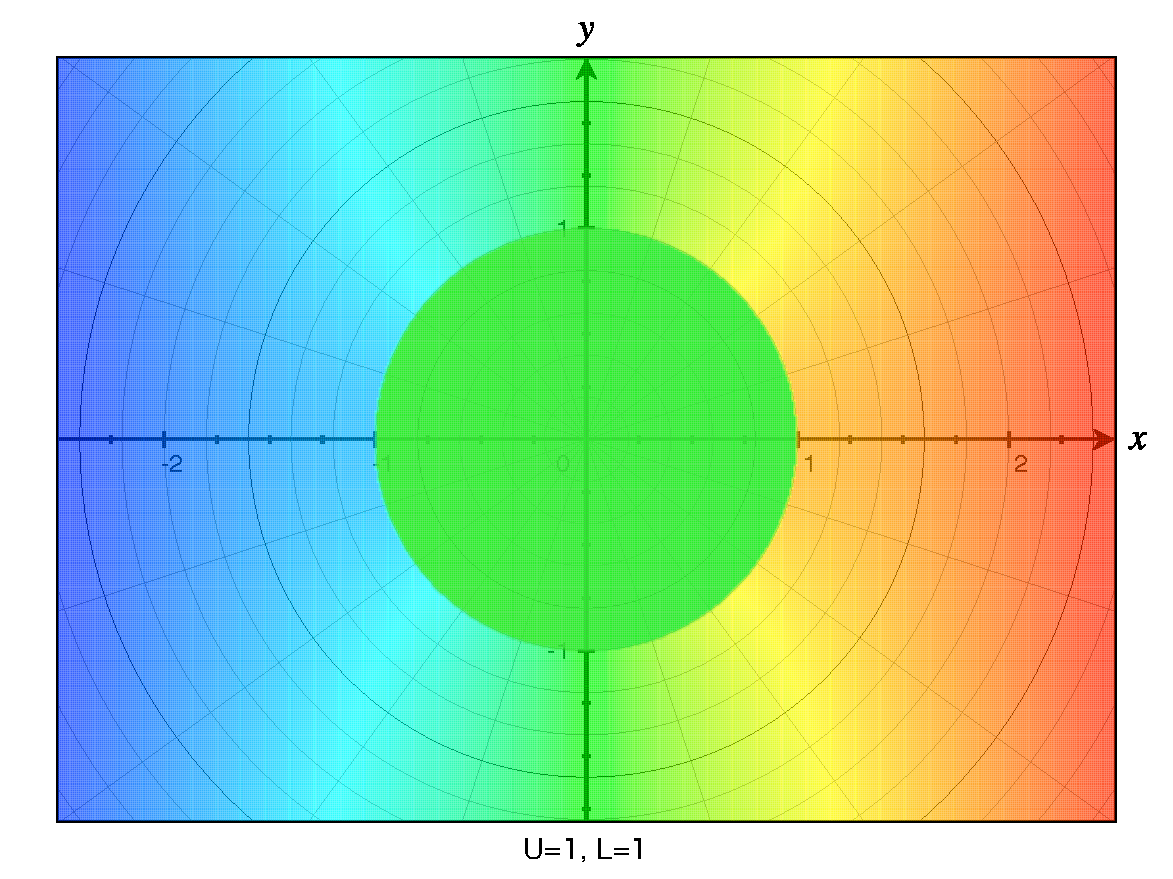
\includegraphics[scale=0.4]{POTENTIAL_U1L1.pdf}
	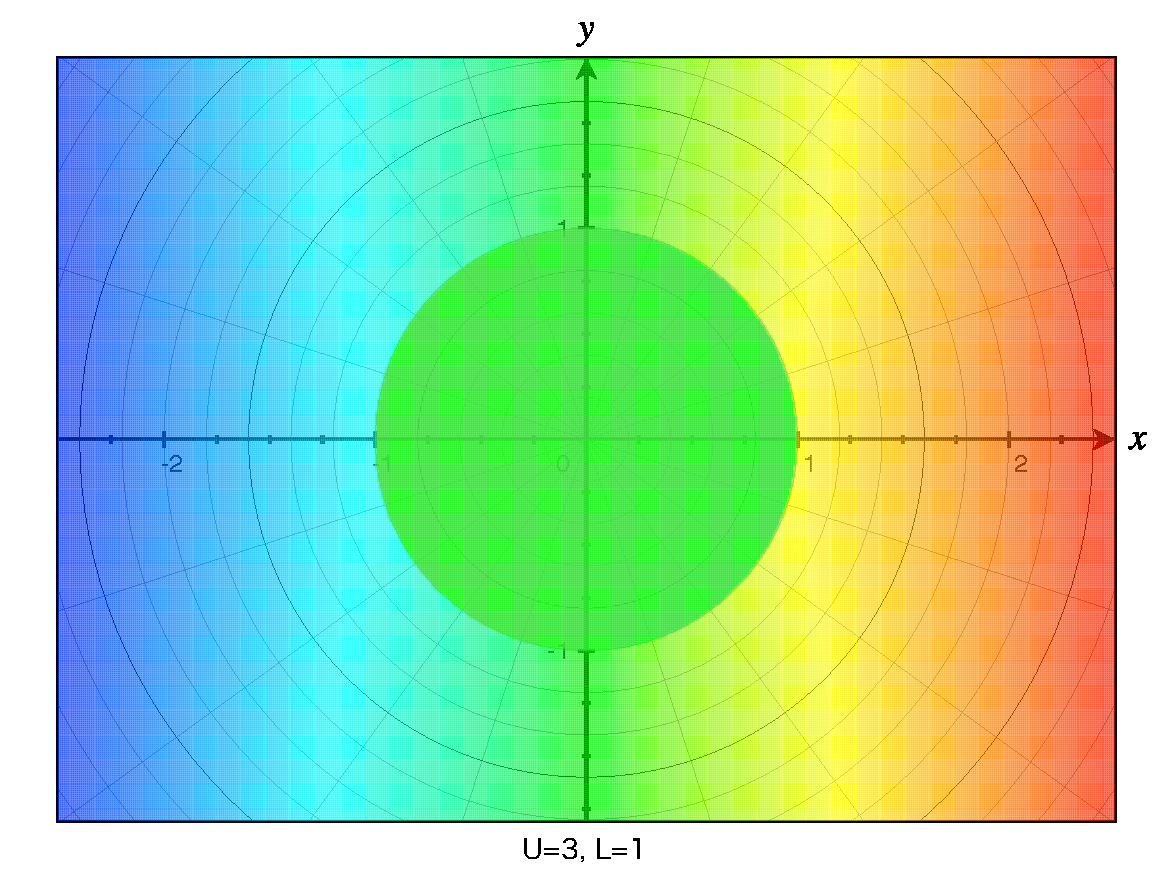
\includegraphics[scale=0.4]{POTENTIAL_U3L1.pdf}
	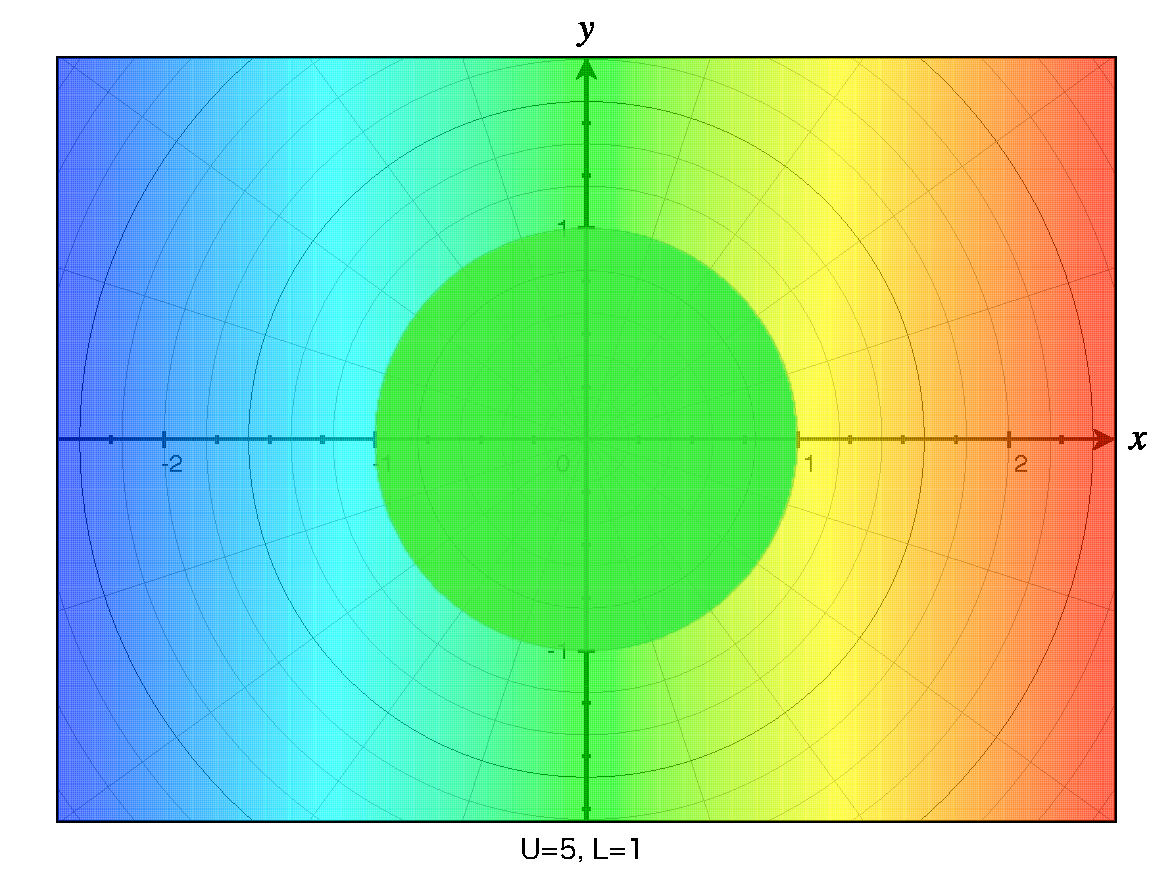
\includegraphics[scale=0.4]{POTENTIAL_U5L1.pdf}
	\caption{Velocity potential plotted for $U\in\{1,3,5\}$ and $L=1$. Blue represents lower values and red represents higher values.}
	\label{figure:VELOCITY-POTENTIAL}
\end{figure}

\subsubsection{The velocity field}
\begin{figure}
	\centering
	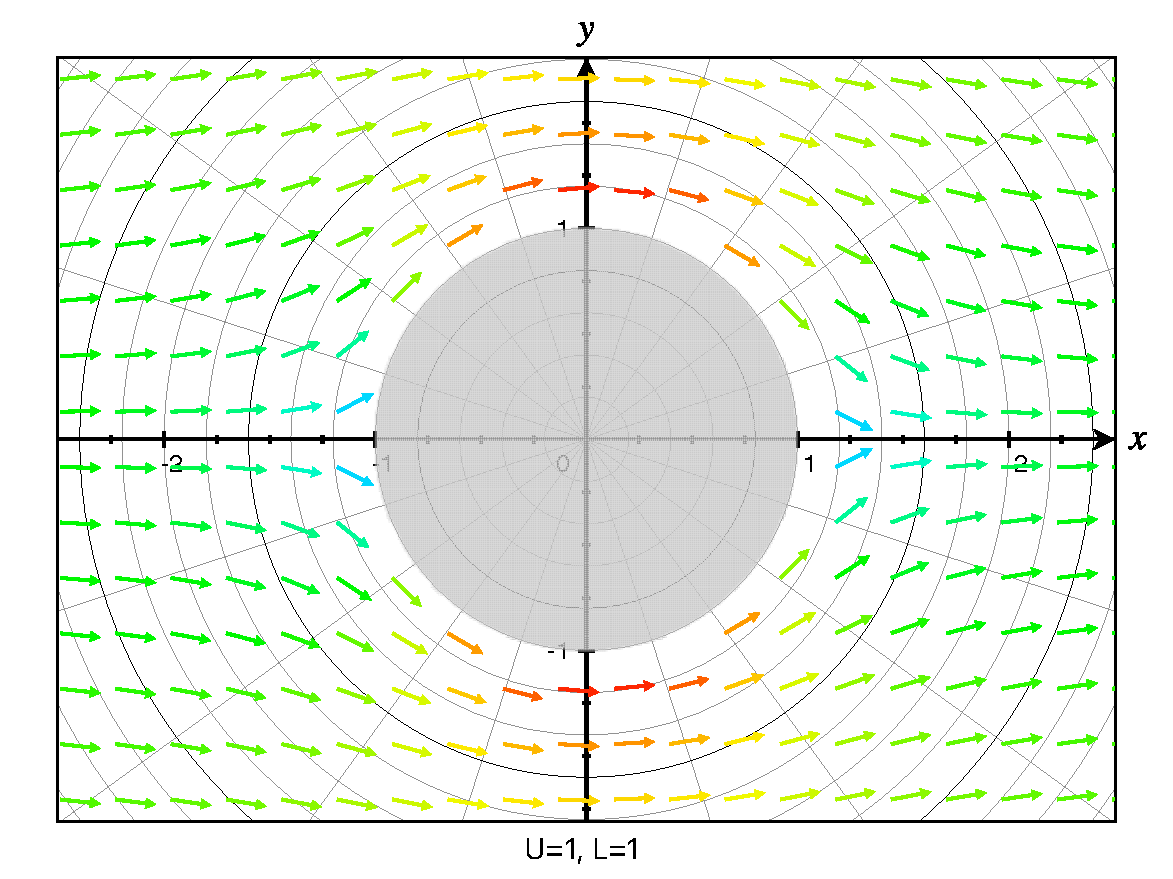
\includegraphics[scale=0.5]{U1L1.pdf}
	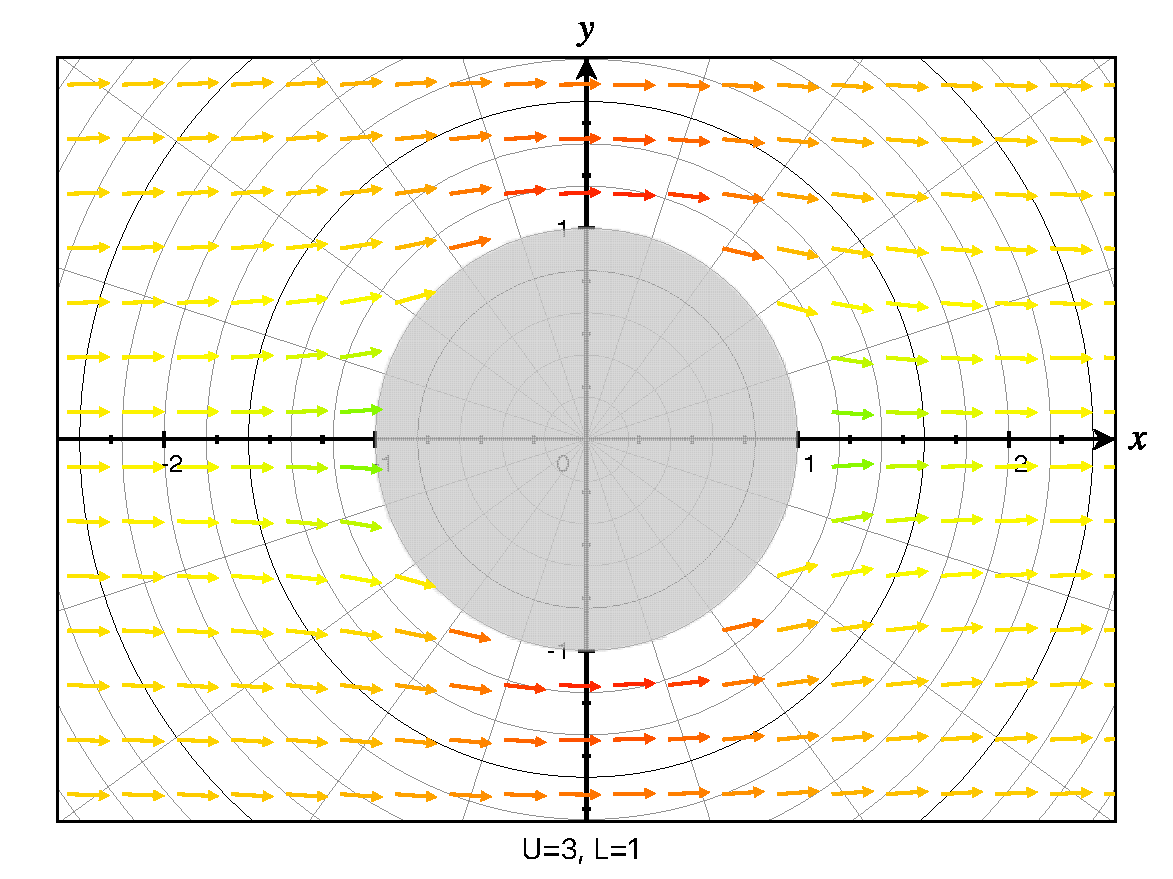
\includegraphics[scale=0.5]{U3L1.pdf}
	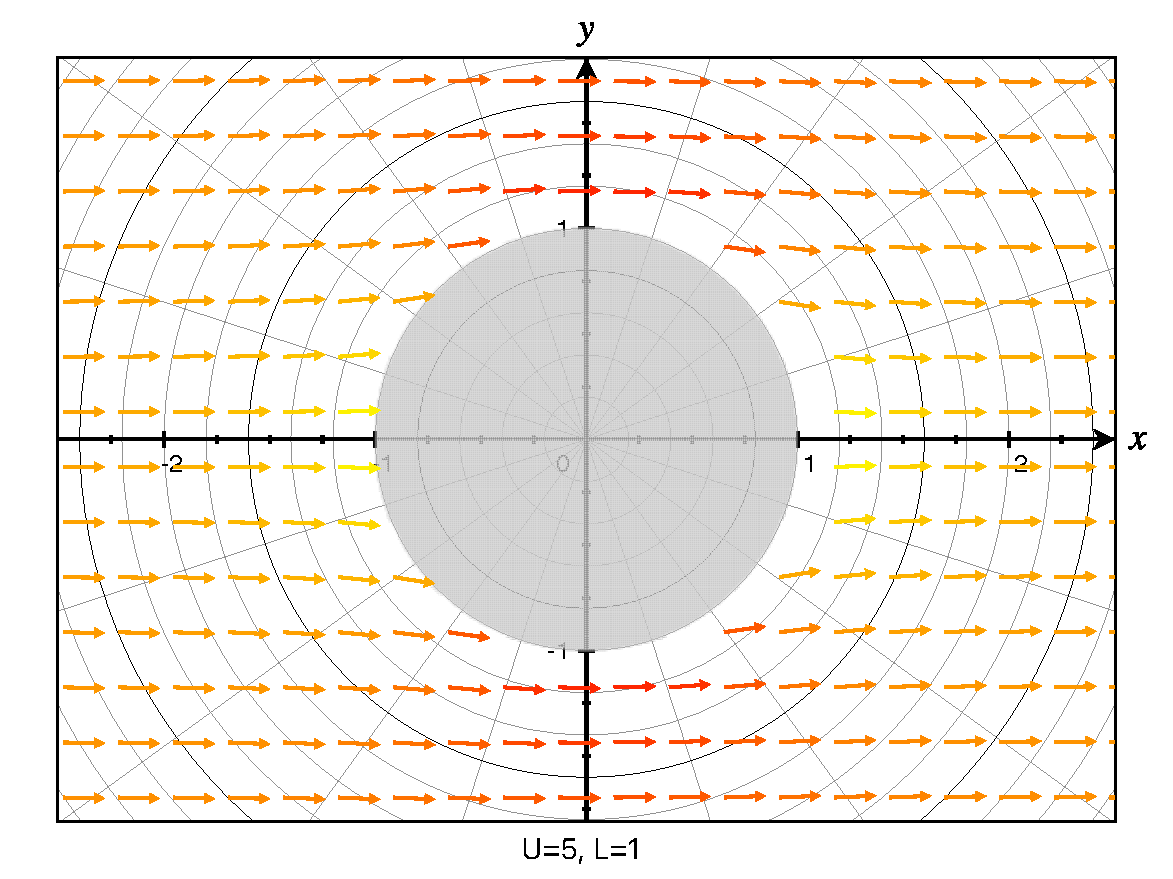
\includegraphics[scale=0.5]{U5L1.pdf}
	\caption{Velocity field plotted for $U\in\{1,3,5\}$ and $L=1$. Blue represents lower speed and red represents higher speed.}
\end{figure}
\begin{figure}
	\centering
	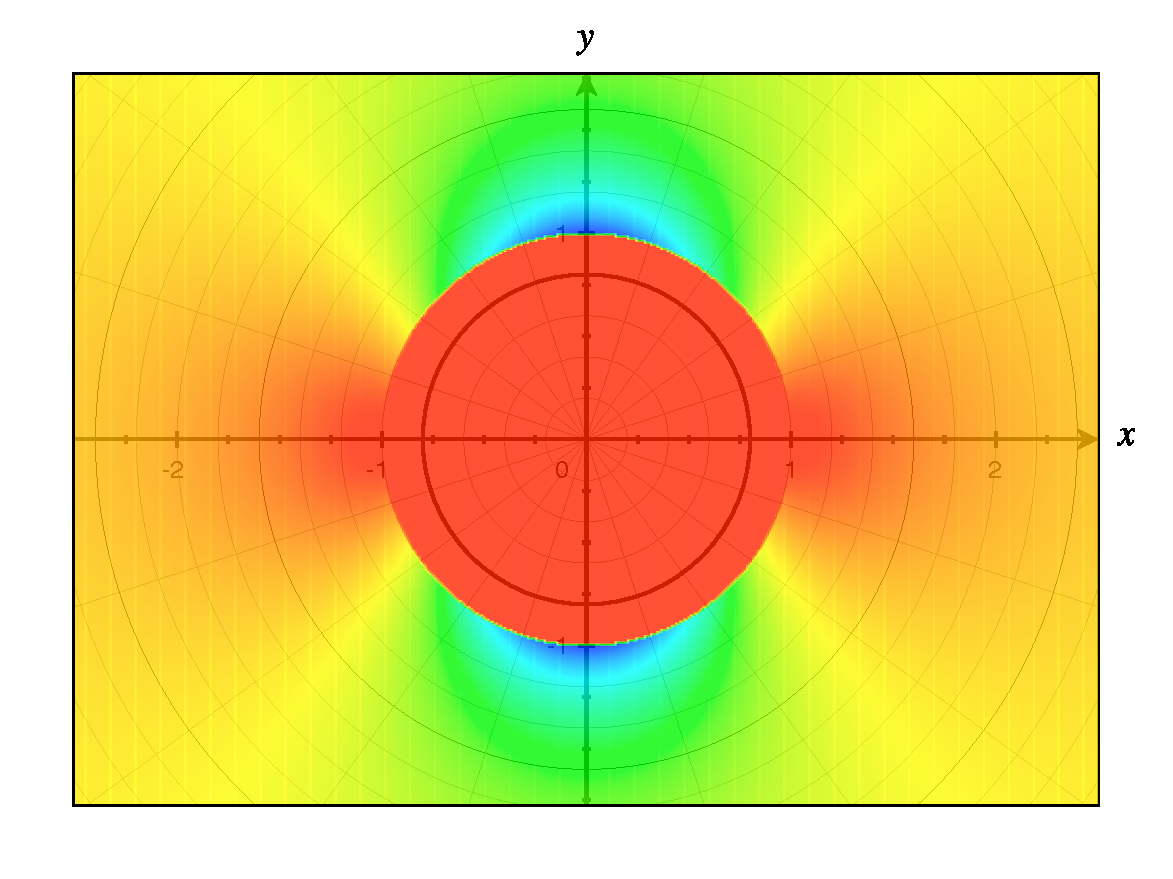
\includegraphics[scale=0.5]{pressure.pdf}
	\caption{Pressure field plotted for $U=L=1$. Blue represents lower pressure and red represents higher pressure.}
\end{figure}
\begin{figure}
	\centering
	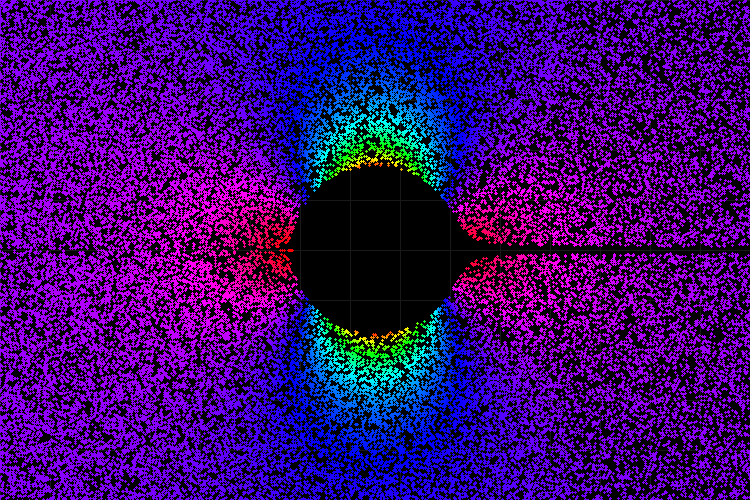
\includegraphics[scale=0.5]{FSim_frame_1.png}
	\caption{Selected frame from a fluid simulation showing a wake forming behind the cylinder. Red-magenta represents lower speed, green-yellow represents higher speed.}
\end{figure}
\begin{figure}
	\centering
	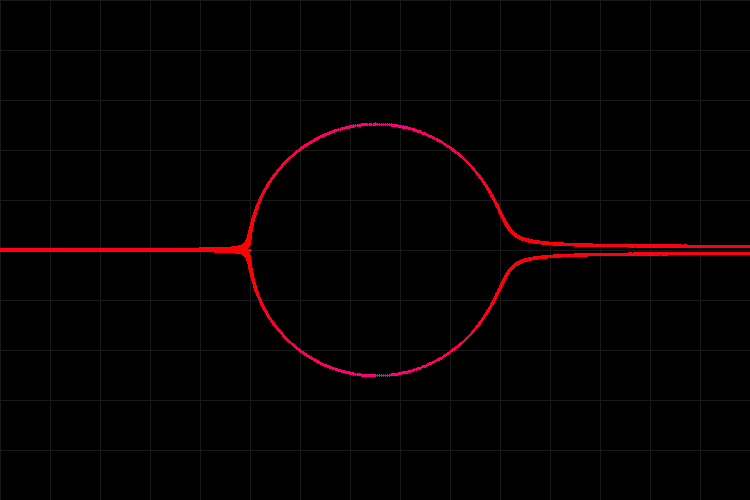
\includegraphics[scale=0.5]{FSim_frame_2.png}
	\caption{Selected frame from a fluid simulation with a narrow distribution of particles around $y=0$, demonstrating wake formation behind the cylinder.}
\end{figure}

\section{Conclusion}